\documentclass[10pt,a4paper]{article}


% Nota:
% A0 bounding box: portrait 0 0 2383 3370
% A0 bounding box: landscape 0 0 3370 2383
% A4 bounding box: portrait 0 0 595 841
% A4 bounding box: landscape 0 0 841 595

% Para multiplas colunas, use o multicolumn

% \usepackage[utf8x]{inputenc}

\usepackage[brazil]{babel}
%\usepackage[latin1]{inputenc}
\usepackage[lmargin=2cm, rmargin=2cm, tmargin=2cm, bmargin=2cm]{geometry} % acerto de margens

\usepackage{multicol}
\usepackage{graphicx}


\usepackage[scaled=.92]{helvet} % font adjusted for times size.

\usepackage{courier} %for typewriter

% espacamento entre colunas
\setlength{\columnsep}{1.5cm}

\pagestyle{empty} % sem enumeracao
\begin{document}

 % \large % usando tamanho grande
\begin{center}
\scalebox{2}{\scshape Rede Emancipa - Simulado}
\end{center}

\section*{Instru\c{c}\~{o}es}
	\begin{enumerate}
	\item  Confira se, al\'em deste caderno, voc\^{e} recebeu o cart\~{a}o destinado \`as respostas. Caso n\~{a}o tenha recebido, pe\c{c}a ao fiscal.
	\item Verifique se este caderno cont\'em 46 quest\~{o}es e uma proposta de reda\c{c}\~{a}o.
	\item Utilize apenas caneta esferogr\'afica azul ou preta.
	\item Cada quest\~{a}o proposta apresenta somente uma alternativa correta. No cart\~{a}o de respostas, atribuir-se-\'a pontua\c{c}\~{a}o zero a toda quest\~{a}o com mais de uma alternativa assinalada, ainda que dentre elas se encontre a correta.
	\item N\~{a}o \'e permitido fazer uso de instrumentos auxiliares para o c\'alculo ou portar material que sirva de consulta.
	\item O tempo dispon\'ivel para esta prova, incluindo o preenchimento do cart\~{a}o de respostas e a realiza\c{c}\~{a}o da reda\c{c}\~{a}o, \'e de cinco horas. Reserve os vinte minutos finais para preencher o cart\~{a}o de respostas.
	\item Quando terminar, entregue ao fiscal o cart\~{a}o de respostas, que poder\'a ser invalidado caso n\~{a}o esteja assinado.
	\item Em caso de d\'uvidas sobre como proceder, pe\c{c}a para falar com o fiscal. N\~{a}o ser\~{a}o esclarecidas quest\~{o}es relativas ao conte\'udo da prova.
	\end{enumerate}

\section*{Proposta de Reda\c{c}\~ao}
	Com base na leitura dos textos motivadores seguintes e nos conhecimentos constru\'idos ao longo de sua forma\c{c}\~{a}o, redija um texto dissertativo-argumentativo em norma culta escrita da l\'ingua portuguesa sobre o tema \textbf{O indiv\'iduo frente \`a \'etica nacional}, apresentando proposta de a\c{c}\~{a}o social, que respeito os direitos humanos. Selecione, organize e relacione coerentemente argumentos e fatos para a defesa do seu ponto de vista. \\

\begin{figure}[!ht]
	\centering
     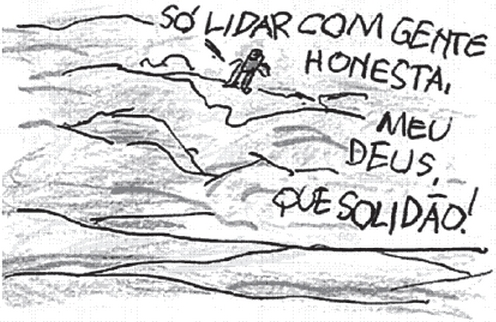
\includegraphics[scale=0.6]{redacao.jpg}
     \caption{Mill\^{o}r Fernandes, dispon\'ivel em uol.com.br/millor/, acessado em 14 jul 2009}
     \label{redacao}
\end{figure}


Andamos demais acomodados, todo mundo reclamando em voz baixa como se fosse errado indignar-se. Sem ufanismo, que dele estou cansada, sem dizer que este \'e um pa\'is rico, de gente boa e cordata, com natureza (a que sobrou) bel\'issima e generosa - sem fantasiar nem botar \'oculos cor-de-rosa que o momento n\~ao permite, eu me pergunto o que anda acontecendo com a gente. \\
 Tenho medo disso que nos tornamos ou em que estamos nos transformando, achando bonita a ignor\^ancia eloquente, engra\c{c}{c}ado o cinismo bem-vestido, interessante o banditismo arrojado, normal o abismo em cuja beira nos equilibramos - n\~ao malabaristas, mas palha\c{c}os. \footnote{LUFT, Ponto de Vista, Ed. 1988, 27 de dezembro de 2006 (adapta\c{c}\~ao)} \\ \\

\textbf{Qual \'e o efeito em n\'os do ``eles s\~ao todos corruptos" ?} \\
As den\'uncias que assolam nosso cotidiano podem dar lugar a uma vontade de transformar o mundo s\'o se nossa indigna\c{c}\~ao n\~ao afetar o mundo inteiro. ``Eles s\~ao TODOS corruptos" ? um pensamento que serve apenas para "confirmar" a "integridade" de quem se indigna. \\
O lugar-comum sobre a corrup\c{c}\~ao generalizada n\~ao \'e uma armadilha para os corruptos: eles continuam iguais e livres, enquanto, fechados em casa, festejamos nossa esplendorosa retid\~ao. \\
O dito lugar-comum \'e uma armadilha que amarra e imobiliza os mesmos que denunciam a imperfei\c{c}{c}\~ao do mundo inteiro. \footnote{CALLIGARIS, C. A armadilha da corrup\c{c}\~ao. Dispon\'ivel em www.folha.uol.com.br (adaptado)} \\ \\

\textbf{INSTRU\c{C}\~OES} \\
\begin{enumerate}
\item Seu texto tem de ser escrito \emph{\`a tinta}, na \emph{folha pr\'opria}.
\item Desenvolva seu texto em prosa: n\~ao redija narra\c{c}\~ao, nem poema.
\item O texto com at\'e 7 (sete) linhas escritas ser\'a considerado em branco.
\item O texto deve ter no m\'aximo \emph{30 linhas}.
\item O \emph{rascunho} da reda\c{c}\~ao dever ser feito no lugar apropriado.
\end{enumerate}


\section*{Quest\~{o}es}
\begin{multicols}{2}


	

\begin{enumerate}

	% in\'icio da qust\~{a}o
	\item \textbf{Texto para esta quest\~{a}o e para a pr\'oxima}\\
	Em 2008, de acordo com o IBGE, 2,4\% dos brasileiros de 7 a 14 anos ainda estavam fora da escola. Embora pare\c{c}a pouco, os n\'umeros absolutos ainda assustam. “S\~{a}o 680 mil crian\c{c}as sem estudar, das quais 450 mil s\~{a}o negras e pardas, a maioria vivendo nas Regi\~{o}es Norte e Nordeste”, revela o soci\'ologo e presidente da Associa\c{c}\~{a}o dos Docentes da Universidade Federal do Amazonas (Ufam) Antônio Neto, para quem esse \'e mais um item a justificar o investimento de 10\% no PIB na educa\c{c}\~{a}o p\'ublica. \footnote{Fonte: http://redeemancipa.org.br/2012/05/entidade-defende-10-do-pib-para-educacao/} \\ \\
O total de brasileiros com idade entre 7 e 14 anos em 2008, de acordo com o IBGE foi de aproximadamente:
		\begin{enumerate}
		\item 3000 mil
		\item 2833 mil
		\item 3 milh\~{o}es
		\item 283 milh\~{o}es
		\item 28 milh\~{o}es
		\end{enumerate}
	% fim da quest\~{a}o

	\item Dentre as 680 mil crian\c{c}as sem estudar, a porcentagem de negras e pardas \'e de aproximadamente:

		\begin{enumerate}
		\item 7\%
		\item 37\%
		\item 53\%
		\item 66\%
		\item 82\%
		\end{enumerate}

	\item No livro ``O homem que calculava", de Malba Tahan, o calculista Beremiz apresenta a defini\c{c}\~{a}o do que seria um n\'umero perfeito da seguinte maneira: "\'e o n\'umero que apresenta a propriedade de ser igual \'e soma de seus divisores, excluindo-se, \'e claro, o pr\'oprio n\'umero. Assim, por exemplo, o n\'umero 28 apresenta 5 divisores menores que 28 (a saber, 1, 2, 4, 7 e 14). \\
	A soma desses divisores ($1+2+4+7+14$) \'e precisamente igual a 28. Logo, 28 pertence \`a  categoria dos n\'umeros perfeitos``. \\
	Qual dos n\'umeros abaixo tamb\'em \'e um \textbf{n\'umero perfeito}?

		\begin{enumerate}
		\item 3
		\item 6
		\item 12
		\item 24
		\item 48
		\end{enumerate}

	\item Joana foi, pela primeira, vez na manifesta\c{c}\~{a}o do 8 de mar\c{c}o (dia internacional da luta das mulheres). L\'a, ela viu um enorme cartaz com dizeres que fez com que ela sentisse muito bem. Segue, abaixo o cartaz com sua medidas:

\begin{figure}
     \centering
     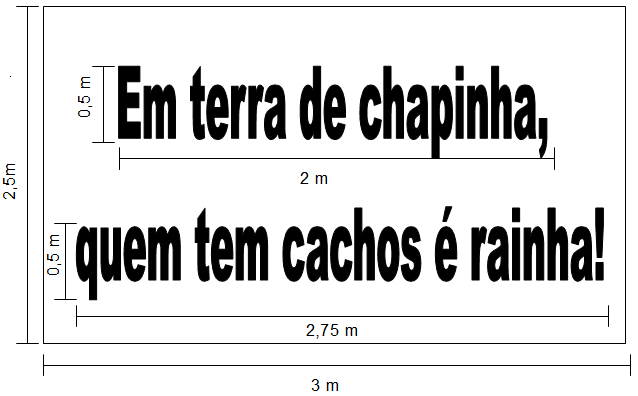
\includegraphics[scale=0.1]{cartaz.png}
     \caption{Cartaz visto por Joana}
     \label{cartaz_joana}
\end{figure}

Chegando em casa, Joana quis fazer uma capa para seu caderno com os mesmos dizeres. Sabendo que a capa do caderno tem 15 cm de altura por 18 cm de comprimento, para manter a propor\c{c}\~{a}o do cartaz, qual deve ser a altura e o comprimento, em cm, da primeira frase (``Em terra de rainha,") e da segunda frase ("quem tem cachos \'e rainha!"), respectivamente?

		\begin{enumerate}
		\item 2 por 12 e 2 por 16,5
		\item 3 por 12 e 3 por 15,5
		\item 3 por 12 e 3 por 16,5
		\item 3 por 15 e 3 por 16,5
		\item 4 por 15 e 4 por 18,5
		\end{enumerate}

	\item Dos 190 candidatos a prefeito nas 26 capitais brasileiras registrados no Tribunal Superior Eleitoral (TSE), apenas 28 (15\%) são mulheres. Segundo o TSE, foram feitos 198.745 registros de homens e 85.893 de mulheres para disputar vagas em todas as Câmaras Municipais do país. Para o cargo de vereador a lei impõe que cada legenda tenha “o mínimo de 30\% e o m\'aximo de 70\% para as candidaturas de cada sexo”. \footnote{Fonte: http://www.tse.jus.br/} \\
	Se todas as candidatas e candidatos a vereadores fossem do mesmo partido a lei citada acima estaria sendo seguida?

		\begin{enumerate}
		\item sim, pois 69,8\% dos candidatos são homens e 30,2\% são mulheres.
		\item sim, pois 67,8\% dos candidatos são homens e 33,1\% são mulheres.
		\item não, pois 72,1\% dos candidatos são homens e 27,9\% são mulheres.
		\item não, pois 33,1\% dos candidatos são homens e 67,8\% são mulheres.
		\item não, pois 30,2\% dos candidatos são homens e 69,8\% são mulheres.
		\end{enumerate}


	%%%  Química
	\item Tem-se uma mistura de magn\'esio e bismuto pulverizados. A densidade (quantidade de massa por volume) do magn\'esio \'e 1,74 g/ml (gramas por $10^{-3}$ litros) e a do bismuto \'e 9,67 g/ml. \\
	Para separar somente esses dois metais, precisamos escolher um líquido adequado. \\
	Assinale a alternativa correta que diz respeito a este líquido:
		\begin{enumerate}
		\item O líquido deve reagir com ambos os metais e tem densidade 2,89 g/ml.
		\item O líquido deve reagir com um dos metais e tem densidade 2,89 g/ml.
		\item O líquido não reage com nenhum dos dois metais e tem densidade 2,89 g/ml.
		\item O líquido pode reagir com um dos metais e tem densidade 1,24 g/ml.
		\item O líquido não reage com nenhum dos metais e tem densidade 1,24 g/ml.
		\end{enumerate}

	\item O n\'umero de el\'etrons do c\'ation (íons de carga positiva) $X^{2+}$ (lembre que cargas positivas são “falta” de el\'etrons) de um elemento X \'e igual ao n\'umero de el\'etrons do \'atomo neutro de um g\'as nobre. Esse \'atomo de g\'as nobre apresenta n\'umero atômico 10 (logo este g\'as nobre tem a seguinte configura\c{c}ão 1$s^2$, 2$s^2$  e 2$p^6$) e n\'umero de massa 20. O n\'umero atômico do elemento X \'e:
		\begin{enumerate}
		\item 8
		\item 10
		\item 12
		\item 18
		\item 20
		\end{enumerate}

	\item O átomo constituído de 17 prótons, 18 nêutrons e 17 elétrons, possui número atômico e número de massa igual a:
		\begin{enumerate}
		\item 17 e 17
		\item 17 e 18
		\item 18 e 17
		\item 17 e 35
		\item 35 e 17
		\end{enumerate}

	\item Na siderurgia, nos altos fornos, ocorre a reação do óxido de ferro ($Fe_2O_3$) com monóxido de carbono (CO). Os processos envolvidos são muito complicados, mas de forma simplificada este processo é realizado segundo a equação:
		$$ Fe_2O_3 \ (s) + 3 CO \ (g) \rightarrow 2Fe \ (s) + 3 CO_2 \ (g) $$
onde (s) indica sólido e (g) indica gás. \\
Obs.: O oxigênio adora ficar com mais dois elétrons para atingir uma configuração de gás nobre. \\
É incorreto afirmar:
		\begin{enumerate}
		\item $Fe_2O_3$ é o agente oxidante.
		\item CO é o agente redutor.
		\item O ferro sofre redução.
		\item O carbono sofre oxidação.
		\item Cada átomo de ferro perde 3 elétrons no processo.
		\end{enumerate}

	%%%%%%%%%%%%%%%%%%%%%%%%%%%%%%%%%%%%%%%%%%%%%%%%
	%%%%%%%%%%%%   Física

	\item O metano é um gás nocivo à atmosfera terrestre por agravar o efeito estufa. Com base no gráfico abaixo, assinale a alternativa correta.

\begin{figure}
     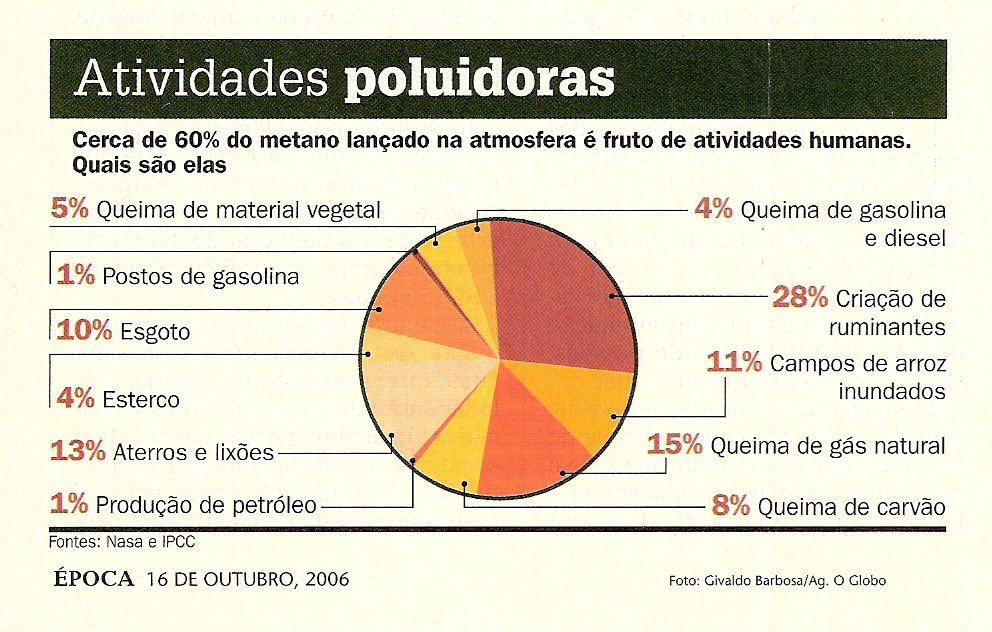
\includegraphics[scale=0.1]{ozonio.jpg}
     \caption{Atividades poluidoras}
     \label{poluidoras}
\end{figure}


		\begin{enumerate}
		\item A emissão de metano devido à criação de ruminantes é maior que a emissão de metano devido a queima de gás natural e carvão juntas
		\item O esterco emite mais metano que a queima de apenas óleo diesel
		\item A produção de petróleo está entre as atividades que mais liberam metano na atmosfera
		\item 40\% do metano lançado na atmosfera é fruto de atividades humanas
		\item A criação de ruminantes é a atividade que menos libera metano na atmosfera
		\end{enumerate}

	\item Apesar de ser um país com enorme oferta de recursos naturais, o Brasil enfrenta problemas de energia elétrica. Com base no gráfico abaixo, é correto afirmar que:

\begin{figure}
     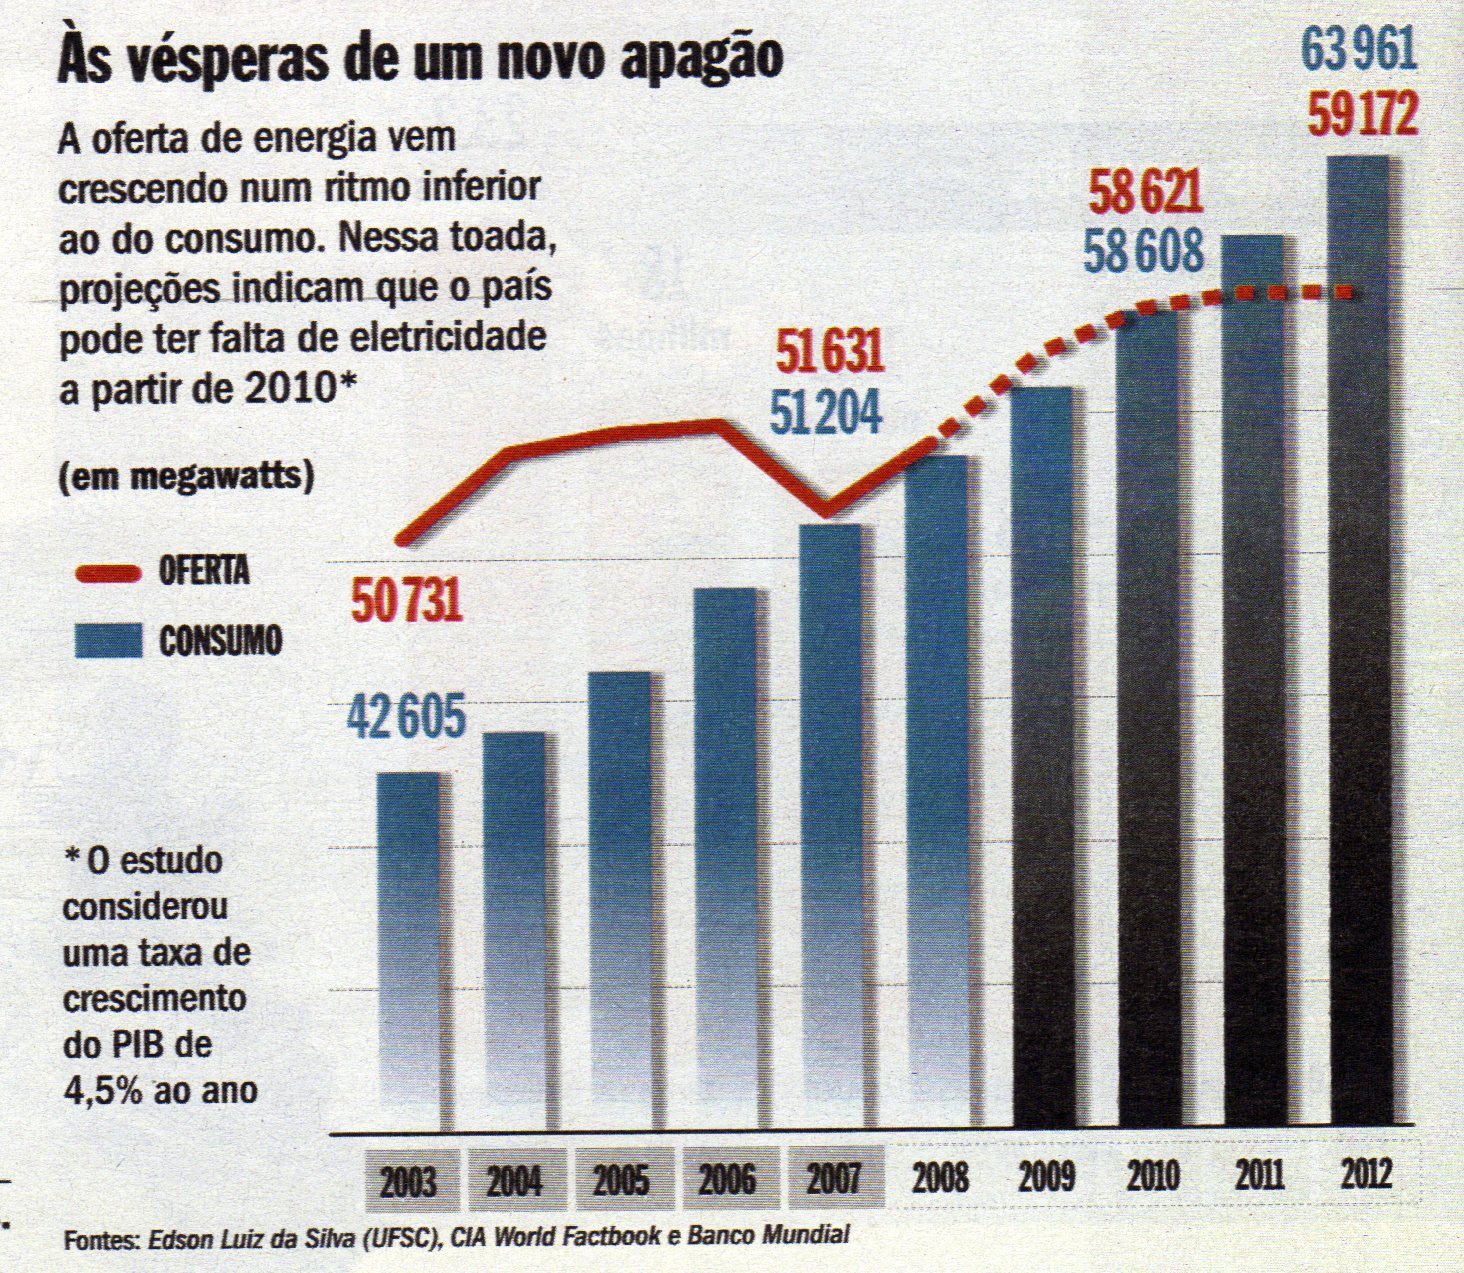
\includegraphics{apagao.jpg}
     \caption{Comparação entre oferta de energia e consumo.}
     \label{energia}
\end{figure}


		\begin{enumerate}
		\item A oferta de energia elétrica era maior em 2007 que em 2006.
		\item A oferta de energia sempre esteve abaixo do consumo.
		\item Em 2005, o consumo de energia era de 50731 megawatts.
		\item O consumo de energia sempre aumentou.
		\item Segundo as previsões, o país poderá ter um apagão a partir de 2012.
		\end{enumerate}


	\item  Em meio às turbulências vividas na primeira metade dos anos 1960, tinha-se a impressão de que 
as tendências de esquerda estavam se fortalecendo na área cultural. O Centro Popular de Cultura (CPC) da União Nacional dos Estudantes (UNE) encenava peças de teatro que faziam agitação e propaganda em favor da luta pelas reformas de base e satirizavam  o ``imperialismo" e seus ``aliados internos". \\
	\emph{KONDER, L. História das Ideias Socialistas no Brasil. São Paulo: Expressão Popular, 2003.}\\
	No início da década de 1960, enquanto vários setores da esquerda brasileira consideravam 
que o CPC da UNE era uma importante forma de conscientização das classes trabalhadoras, 
os setores conservadores e de direita (políticos vinculados à União Democrática Nacional - UDN -, 
Igreja Católica, grandes empresários, etc) entendiam que esta organização:
		\begin{enumerate}
		\item constituía mais uma ameaça para a democracia brasileira, ao difundir a ideologia comunista.
		\item contribuía com a valorização da genuína cultura nacional, ao encenar peças de cunho popular.
		\item realizava uma tarefa que deveria ser exclusiva do Estado, ao pretender educar o povo por meio da cultura.
		\item prestava um serviço importante à sociedade brasileira, ao incentivar a participação política dos 
mais pobres.
		\item diminuía a força dos operários urbanos, ao substituir os sindicatos como instituição de pressão política sobre o governo.
		\end{enumerate}


	\item É difícil encontrar um texto sobre a Proclamação  da republica no Brasil que não cite a afirmação de Aristides Lobo, no Diário Popular de São Paulo, de que ``o povo assistiu àquilo bestializado". Essa versão foi relida pelos enaltecedores da Revolução de 1930, que não descuidaram da forma republicana, mas realçaram a exclusão social, o militarismo e o estrangeirismo da fórmula implantada em 1889. Isto porque o Brasil brasileiro teria nascido em 1930. \footnote{MELLO, M. T. C. A república consentida:cultura democrática e cientifica no final do impérioRio de Janeiro: FGV, 2007 (adaptado).} \\
	O texto defende que a consolidação de uma determinada memória sobre a Proclamação da República no Brasil teve, na Revolução de 1930, um de seus momentos mais importantes. Os defensores da Revolução de 1930 procuraram construir uma visão negativa para os eventos de 1889, porque esta era uma maneira de
		\begin{enumerate}
		\item valorizar as propostas políticas democráticas e liberais vitoriosas.
		\item resgatar simbolicamente as figuras politicas ligadas à Monarquia.
		\item criticar a política educacional adotada durante a República Velha.
		\item legitimar a ordem política inaugurada com a chegada desse grupo ao poder.
		\item destacar a ampla participação popular obtida no processo da Proclamação.
		\end{enumerate}


	\item Completamente analfabeto, ou quase, sem assistência médica, não lendo jornais, nem revistas,
 nas quais se limita a ver figuras, o trabalhador rural não ser em casos esporádicos, tem o patrão na conta 
de benfeitor. No plano político, ele luta com o ``coronel" e pelo ``coronel". Aí estão os votos de cabresto, que resultam, em grande parte, da nossa organização econômica rural. \footnote{LEAL, V. N. Coronelismo, enxada e voto. São Paulo: Alfa-Ômega, 1978 (adaptado).} \\
	O coronelismo, fenômeno político da Primeira República (1889-1930), tinha como uma de suas principais características o controle do voto, o que limitava, portanto, o exercício da cidadania. Nesse período, esta prática estava vinculada a uma estrutura social

		\begin{enumerate}
		\item igualitária, com um nível satisfatório de distribuição da renda.
		\item estagnada, com uma relativa harmonia entre as classes.   
		\item tradicional, com a manutenção da escravidão nos engenhos como forma produtiva típica.
		\item ditatorial, perturbada por um constante clima de opressão mantido pelo exército e polícia.
		\item agrária, marcada pela concentração da terra e do poder político local e regional.
		\end{enumerate}


	\item
		\begin{enumerate}
		\item 
		\item 
		\item 
		\item 
		\item 
		\end{enumerate}




\end{enumerate}
\end{multicols}

% \vspace{2pc} \hrule \vspace{1pc} \hrule

\end{document}
